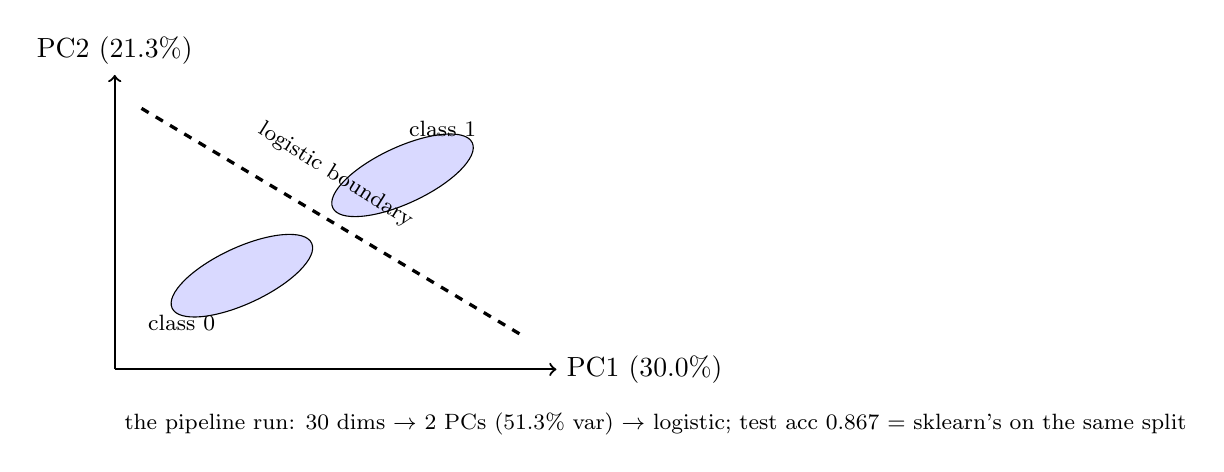
\begin{tikzpicture}[scale=0.85]
% schematic 2D PCA projection + logistic boundary on the pipeline's
% real numbers (var explained .300/.213, test acc .867)
\draw[->, thick] (0,0) -- (6.6,0) node[right] {PC1 (30.0\%)};
\draw[->, thick] (0,0) -- (0,4.4) node[above] {PC2 (21.3\%)};
% two elongated blobs, boundary along y = -0.5x + 0.4 roughly
\foreach \dx/\dy/\rot in {4.3/2.9/25, 1.9/1.4/25}{
  \draw[fill=blue!15, rotate around={\rot:(\dx,\dy)}]
    (\dx,\dy) ellipse (1.15 and 0.42);}
\node[font=\footnotesize] at (4.9,3.6) {class 1};
\node[font=\footnotesize] at (1.0,0.7) {class 0};
\draw[very thick, dashed] (0.4,3.9) -- (6.1,0.5);
\node[font=\footnotesize, rotate=-32] at (3.3,2.9)
  {logistic boundary};
\node[align=left, anchor=north west] at (0,-0.5) {\footnotesize
  the pipeline run: 30 dims $\to$ 2 PCs (51.3\% var) $\to$ logistic;
  test acc 0.867 = sklearn's on the same split};
\end{tikzpicture}
